% \documentclass[./main.tex]{subfiles}
% \graphicspath{ {/images/} 

\begin{document}
% \begin{center}
\subsection{ESP32}
   Mikrokontrolér  pripojiteľný na Wi-Fi alebo bluetooth
   
\begin{wrapfigure}[8]{r}[-9mm]{0.45\textwidth }
    \centering
  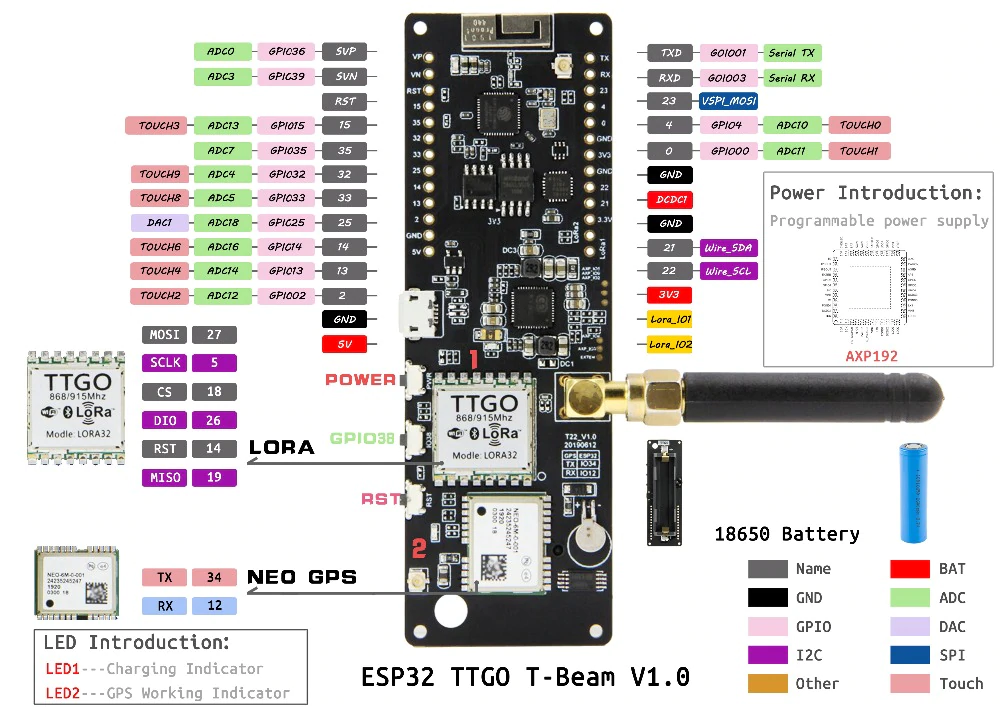
\includegraphics[width= 0.43\textwidth ]{esp32-tbeam.png}
  \caption{ESP32-tbeam}
\end{wrapfigure}

            \paragraph{Robustný dizajn} je odolný s operačnou teplotou –40°C to +125°C. Je výhodný do priemyselného prostredia. Je schopný odstrániť nedokonalosti obvodov a adaptovať sa na extrémne podmienky vďaka posilneným kalibračným obvodom.
            \paragraph{Vysoký level integrácie} je spojený so vstavanými prepínačmi antény, RF symetrizačným členom, zosilňovačom, filtrami a spotrebnými modulami.
            \paragraph{Ultra-nízka spotreba} - je vhodný pre mobilné zariadenia, IoT aplikácie a do prenosnej elektroniky.
            \paragraph{Hybrid Wi-Fi \& Bluetooth Chip} - môže fungovať samostatne alebo po mikrokontrolérom. Môže byť prepojené s inými systémami na poskytovanie Wi-Fi a Bluetoothu cez SPI \/ SDIO or I2C \/ UART rozhrania.
    
\subfile{sections/esp32/heltec_lora32.tex}
% \subfile{sections/esp32/micropython.tex}

% \end{center}
\end{document}